\chapter{METODOLOGI}
\label{chap:metodologi}

% Ubah bagian-bagian berikut dengan isi dari desain dan implementasi

% Penelitian ini dilaksanakan sesuai dengan batasan-batasan masalah yang telah disebutkan
% pada bagian 1.3. Berikut ini adalah beberapa peralatan dan perangkat yang terlibat dalam
% penelitian ini.

\section{Metode yang Digunakan}
\label{sec:metodeyangdigunakan}

Tugas akhir ini merupakan penelitian di bidang visi komputer dengan tujuan untuk melakukan 
re-identifikasi mobil menggunakan kumpulan citra dari dataset VRIC. Alur blok diagram metodologi 
dapat dilihat pada gambar \ref{fig:diagramblokmetodologi}. Pengembangan model menggunakan metode 
Swin Transformer dari \emph{Pytorch ReID layumi}.

\begin{figure}[ht]
  \centering
  % Nama dari file gambar yang diinputkan
  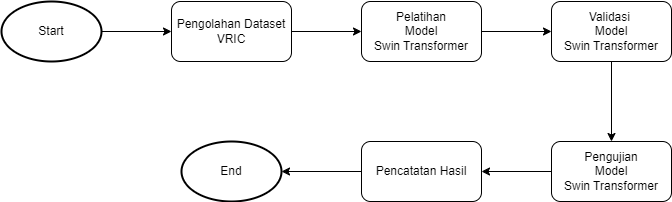
\includegraphics[scale=0.6]{gambar/metodologiUpdate.png}
  % Keterangan gambar yang diinputkan
  \caption{Diagram Blok Metodologi}
  % Label referensi dari gambar yang diinputkan
  \label{fig:diagramblokmetodologi}
\end{figure}

\begin{enumerate}[nolistsep]

  \item \textbf{Pengolahan Dataset VRIC}
  
  Pada tahapan ini, dilakukan proses pengolahan dataset VRIC dengan 
  membagi dataset sesuai kebutuhan dari model. Terdapat tiga tahap yang akan 
  dilalui model, dimana setiap tahapnya membutuhkan data yang berbeda-beda. Tiga 
  tahap tersebut yaitu  tahap \linebreak pelatihan (\emph{training}), tahap validasi 
  (\emph{validation}), dan tahap pengujian (\emph{testing}). Sehingga perlu membaginya 
  sesuai dengan kebutuhan di setiap tahapannya.

  \item \textbf{Pelatihan Model Swin Transformer}
  
  Pada tahapan ini, dilakukan pelatihan (\emph{training}) pada model Swin Transformer 
  menggunakan data \emph{training} VRIC yang telah dibagi dari tahapan sebelumnya. 
  Di tahapan ini juga dilakukan pengaturan hyper-parameter agar mendapatkan nilai akurasi, 
  mAP (\emph{Mean Average Precision}), dan rank@1 yang tinggi.

  \item \textbf{Validasi Model Swin Transformer}
  
  Pada tahapan ini, dilakukan validasi (\emph{validation}) pada model Swin Transformer yang 
  telah selesai pelatihan. Validasi disini menggunakan data \emph{validation} VRIC, sehingga 
  tidak menggunakan data yang sama dengan tahap pelatihan.

  \item \textbf{Pengujian Model Swin Transformer}
  
  Pada tahapan ini, model Swin Transformer yang telah selesai dikembangkan bisa diujicobakan 
  menggunakan data kueri(\emph{query}) dan data galeri (\emph{gallery}) dari VRIC.

  \item \textbf{Pencatatan Hasil}
  
  Model yang telah melalui tahapan pelatihan, validasi, dan dapat diujicobakan, akan 
  dicatat hasil akurasi, mAP, dan rank@1. Terdapat dua belas model yang akan dibandingkan 
  dan nantinya akan diambil kesimpulan model terbaik dari penelitian.

\end{enumerate}

\section{Bahan dan Peralatan yang Digunakan}
\label{sec:bahandanperalatanyangdigunakan}

\subsection{Dataset}

Dataset yang digunakan dalam penelitian ini adalah dataset VRIC. Dataset VRIC memuat 
60 ribu citra mobil yang diambil dari kamera CCTV dari berbagai sudut pandang, sudut 
pencahayaan, dan kondisi lingkungan yang bermacam-macam. Setiap citra mobil dari dataset 
VRIC telah diberikan label sesuai dengan id kendaraan dan id kamera yang mengambil 
citra tersebut.

\begin{figure}[ht]
  \centering
  % Nama dari file gambar yang diinputkan
  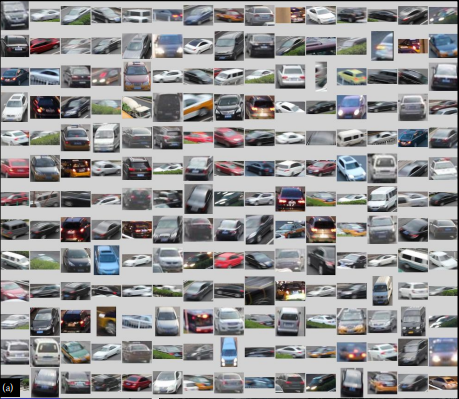
\includegraphics[scale=0.55]{gambar/VRICcontoh.png}
  % Keterangan gambar yang diinputkan
  \caption{Citra pada Dataset VRIC}
  % Label referensi dari gambar yang diinputkan
  \label{fig:citrapadadatasetvric}
\end{figure}

Gambar \ref{fig:citrapadadatasetvric} merupakan beberapa contoh citra yang ada di dataset 
VRIC. Di dalam dataset VRIC,terdapat tiga folder yang telah dibuat, yaitu folder \emph{train}, 
\emph{gallery}, dan \emph{query}. Folder \emph{train} berisikan 54 
ribu citra, sementara pada folder \emph{gallery} dan \emph{query} masing-masing 
berisikan 2 ribu citra. Terdapat pula list anotasi dari seluruh citra yang berisikan 
format nama file citra, label ID dari mobil, dan label kamera.

\subsection{Laptop}

Laptop digunakan untuk melakukan pengolahan dataset, pelatihan model, validasi model, 
dan pengujian model. Laptop perlu terhubung dengan internet untuk mengakses Google \linebreak
Colaboratory, yang merupakan \emph{environment} yang dibutuhkan untuk membuat model Swin 
\linebreak Transformer. Spesifikasi laptop yang digunakan dapat dilihat pada tabel 
\ref{tb:spesifikasilaptop}.

\begin{table}[ht]
  \begin{center}
  \caption{Spesifikasi Perangkat Laptop yang Digunakan}
  \label{tb:spesifikasilaptop}
  \begin{tabular}{|l|l|}
      \hline
      \textit{\textbf{Processor}}        & \begin{tabular}[c]{@{}l@{}}Intel Core i7-8750H \\ CPU @ 2.2 GHz\end{tabular} \\ \hline
      \textit{\textbf{Storage}}          & \begin{tabular}[c]{@{}l@{}}SSHD 1 TB Storage\\ SSD 128 GB Storage\end{tabular}         \\ \hline
      \textit{\textbf{RAM}}              & \begin{tabular}[c]{@{}l@{}}16 GB SODIMM DDR4 \\ 2666 MHz Dual Channel\end{tabular}    \\ \hline
      \textit{\textbf{Graphic Card}}     & \begin{tabular}[c]{@{}l@{}}NVIDIA GeForce GTX 1050 Ti \\ 4 GB GDDR5\end{tabular}      \\ \hline
      \textit{\textbf{Operating System}} & \begin{tabular}[c]{@{}l@{}}Windows 10 Home \\ Single Language 64-bit\end{tabular}     \\ \hline
  \end{tabular}
  \end{center}
\end{table}

\subsection{Google Colaboratory}

Google Colaboratory merupakan sebuah \emph{environment} komputasi cloud dengan format 
\linebreak notebook yang disediakan oleh Google research dengan fungsi untuk 
menjalankan kode python yang telah dituliskan. Google Colaboratory sangat membantu 
dalam pengerjaan \emph{data science}, \emph{deep learning}, dan \emph{machine learning} 
dikarenakan spesifikasi \emph{hardware} yang tinggi dari Google Colaboratory. Spesifikasi 
Google Colaboratory yang digunakan dapat dilihat pada tabel 
\ref{tb:spesifikasigooglecolaboratory}.

\begin{table}[ht]
  \begin{center}
  \caption{Spesifikasi Google Colaboratory}
  \label{tb:spesifikasigooglecolaboratory}
  \begin{tabular}{|l|l|}
      \hline
      \textit{\textbf{Processor}}        & \begin{tabular}[c]{@{}l@{}}Intel(R) Xeon(R) \\ CPU @ 2.2 GHz\end{tabular} \\ \hline
      \textit{\textbf{Graphic Card}}     & \begin{tabular}[c]{@{}l@{}}NVIDIA A100 SXM \\ 40 GB HBM2\end{tabular}      \\ \hline
  \end{tabular}
  \end{center}
\end{table}

\section{Urutan Pelaksanaan Penelitian}
\label{sec:urutanpelaksanaanpenelitian}

\subsection{Pengolahan Dataset}

Dataset VRIC terbagi menjadi tiga bagian, yaitu data \emph{training}, data \emph{query}, 
dan data \emph{gallery}. Ketiga bagian dataset tersebut telah dipisahkan dan disesuaikan 
secara langsung oleh developer dataset VRIC untuk kegunaan re-identifikasi mobil. 
Selain file berisi citra, di dalam dataset VRIC juga terdapat file txt yang berisi list 
anotasi dari seluruh citra, dengan format nama file citra, label ID dari mobil, dan label 
kamera. Dengan menggunakan list anotasi tersebut, maka setiap dataset 
perlu dilakukan perubahan nama file sesuai dengan label ID dan label kameranya.\\

% Potongan kode rename
\lstinputlisting[
  language=Python,
  caption={Program Rename Dataset.},
  label={lst:renamedataset}
]{program/perubahan-nama-file.py}

Pada penelitian ini, diperlukan satu bagian lagi dalam percobaannya, yaitu data validasi. 
Data validasi berfungsi untuk melakukan validasi dan mengetes re-identifikasi setiap epoch yang telah 
melalui tahapan \emph{training}. Data validasi dibuat dengan mengambil sebagian data \emph{training} 
untuk dipindahkan ke data validasi. \\

% Potongan kode splitting
\lstinputlisting[
  language=Python,
  caption={Program Pembagian Dataset.},
  label={lst:splittingdataset}
]{program/splitting-dataset.py}

\subsection{\emph{Training}}

\emph{Training} dilakukan setelah proses perubahan nama dan pemisahan dataset selesai \linebreak dilakukan. 
Di dalam proses \emph{Training}, terdapat beberapa konfigurasi hyper-parameter yang harus 
ditentukan yaitu:

\begin{enumerate}[nolistsep]

  \item \textbf{Epoch}
  
  Epoch adalah hyper-parameter yang berfungsi untuk menentukan jumlah pengulangan proses \emph{learning} 
  yang harus dilakukan algoritma \emph{learning} ke sebuah dataset \emph{training}. Semakin banyaknya 
  pengulangan yang dilakukan maka model yang dihasilkan akan memiliki tingkat akurasi yang semakin 
  tinggi, namun waktu yang dibutuhkan dalam melakukan \emph{training} juga akan semakin banyak.

  \item \textbf{\emph{Batch Size}}
  
  \emph{Batch size} adalah hyper-parameter yang berfungsi untuk mengontrol jumlah sampel \linebreak \emph{training} 
  untuk dikerjakan sebelum parameter internal model diperbarui. Batch dapat dibayangkan seperti \emph{for-loop} 
  yang mengulang beberapa sampel dan kemudian membuat prediksi. Di akhir batch, prediksi dibandingkan 
  dengan variabel keluaran yang diharapkan dan kesalahan akan dihitung. Dari kesalahan ini, maka algoritma 
  pembaruan akan digunakan untuk memperbaiki model. 

  \item \textbf{\emph{Image Size}}
  
  \emph{Image size} merupakan dimensi ukuran citra yang diterapkan pada dataset. Ketika ukuran citra yang 
  diterapkan semakin kecil, maka waktu yang dibutuhkan untuk melakukan proses \emph{training} akan semakin singkat. 

  \item \textbf{\emph{Learning Rate}}
  
  \emph{Learning rate} adalah hyper-parameter yang mengontrol besarnya perubahan suatu model dalam menanggapi 
  estimasi kesalahan setiap kali \emph{weight model} diperbarui. Dibutuhkan pemilihan nilai \emph{learning rate} 
  yang tepat karena ketika nilai yang digunakan terlalu kecil akan berdampak pada proses \emph{training} yang 
  terlalu lama, sementara jika nilai yang digunakan terlalu besar mengakibatkan proses \emph{learning} kurang 
  optimal.


  \item \textbf{\emph{Random Erasing Probability}}
  
  \emph{Random erasing probability} adalah hyper-parameter yang akan secara acak memilih sebagian wilayah dengan 
  bentuk persegi panjang kemudian menghapus pikselnya dengan nilai acak. \emph{Random erasing} melengkapi teknik 
  augmentasi data yang biasa digunakan seperti pemotongan dan pembalikan acak sehingga menghasilkan peningkatan yang 
  konsisten ketika digunakan di klasifikasi gambar, deteksi objek, dan re-identifikasi.

\end{enumerate}

\subsection{\emph{Validation}}

\emph{validation} dilakukan setelah model menyelesaikan tahap \emph{training} pada setiap epochnya. Di dalam proses 
validasi, model akan mencoba melakukan re-identifikasi menggunakan data validasi yang telah dibuat pada tahap 
pengolahan dataset. Sehingga model akan membaca data baru yang berbeda dengan data \emph{training}. Nilai akurasi, 
loss, dan Top 1 Error akan didapatkan setelah tahap validasi selesai.

% \subsection{Model}

% Penelitian ini akan menggunakan Swin Transformer V1 dan Swin Transformer V2 sebagai model dengan varian
% yang akan digunakan adalah varian \emph{Base} (Swin-B). Kemudian akan dicoba pula menggunakan 2 format hyper-parameter yang 
% berbeda. Sehingga akan dihasilkan 4 jenis model re-identifikasi mobil dengan pengaturan yang berbeda. Rincian hyper-parameter 
% dapat dilihat pada \ref{tb:rincianmodeldanhyperparameterdaripenelitian}.

% \begin{table}[ht]
%   \begin{center}
%   \caption{Rincian Model dan Hyper-Parameter dari Penelitian}
%   \label{tb:rincianmodeldanhyperparameterdaripenelitian}
%   \begin{tabular}{|l|l|l|}
%       \hline
%       \textit{ }        & \begin{tabular}[c]{@{}l@{}}\textbf{Swin Transformer V1}\end{tabular} & \begin{tabular}[c]{@{}l@{}}\textbf{Swin Transformer V2}\end{tabular}\\ \hline
%       \textit{\textbf{Parameter 1}}  & \multicolumn{2}{|c|}{\parbox{6cm}{Batch Size=32; \\ Random Erasing Probability=0; \\ Learning Rate=0.05; \\ Warm Epoch=0}} \\ \hline
%       \textit{\textbf{Parameter 2}}  & \multicolumn{2}{|c|}{\parbox{6cm}{Batch Size=16; \\ Random Erasing Probability=0.5; \\ Learning Rate=0.01; \\ Warm Epoch=5}} \\ \hline
%       % \textit{\textbf{Parameter 1}}  & \begin{tabular}[c]{@{}l@{}}Batch Size=32 \\ Random Erasing Probability=0 \\ Learning Rate=0.05 \\ Warm Epoch=0\end{tabular} \\ \hline
%       % \textit{\textbf{Parameter 2}}  & \begin{tabular}[c]{@{}l@{}}Batch Size=16 \\ Random Erasing Probability=0.5 \\ Learning Rate=0.01 \\ Warm Epoch=5\end{tabular} \\ \hline
%   \end{tabular}
%   \end{center}
% \end{table}

\subsection{Pengujian Model}

Setiap model yang dibuat berdasarkan jenis model dan pengaturan hyper-parameternya akan diujicobakan menggunakan data \emph{test} 
(data kueri dan data galeri) dari dataset VRIC yang telah disiapkan. Hasil pengujian dari setiap model
re-identifikasinya akan dibandingkan performanya dan dicatat di penelitian ini. Dari pencatatan ini, nantinya dapat diketahui 
jenis model dan pengaturan hyper-parameter yang tepat untuk digunakan dalam re-identifikasi mobil.

\section{Model Penelitian}
\label{sec:modelpenelitian}

Penelitian ini akan menggunakan Swin Transformer V1 dan Swin Transformer V2 sebagai model dengan varian
yang akan digunakan adalah varian \emph{Base} (Swin-B). Kemudian akan dicoba pula menggunakan 2 format hyper-parameter yang 
berbeda. Sehingga akan dihasilkan 4 jenis model re-identifikasi mobil dengan pengaturan yang berbeda. Rincian hyper-parameter 
dapat dilihat pada \ref{tb:rincianmodeldanhyperparameterdaripenelitian}.

\begin{table}[ht]
  \begin{center}
  \caption{Rincian Model dan Hyper-Parameter dari Penelitian}
  \label{tb:rincianmodeldanhyperparameterdaripenelitian}
  \begin{tabular}{|l|l|l|}
      \hline
      \textit{ }        & \begin{tabular}[c]{@{}l@{}}\textbf{Swin Transformer V1}\end{tabular} & \begin{tabular}[c]{@{}l@{}}\textbf{Swin Transformer V2}\end{tabular}\\ \hline
      \textit{\textbf{Parameter 1}}  & \multicolumn{2}{|c|}{\parbox{6cm}{Batch Size=32; \\ Random Erasing Probability=0; \\ Learning Rate=0,05; \\ Warm Epoch=0}} \\ \hline
      \textit{\textbf{Parameter 2}}  & \multicolumn{2}{|c|}{\parbox{6cm}{Batch Size=16; \\ Random Erasing Probability=0,5; \\ Learning Rate=0,01; \\ Warm Epoch=5}} \\ \hline
      % \textit{\textbf{Parameter 1}}  & \begin{tabular}[c]{@{}l@{}}Batch Size=32 \\ Random Erasing Probability=0 \\ Learning Rate=0.05 \\ Warm Epoch=0\end{tabular} \\ \hline
      % \textit{\textbf{Parameter 2}}  & \begin{tabular}[c]{@{}l@{}}Batch Size=16 \\ Random Erasing Probability=0.5 \\ Learning Rate=0.01 \\ Warm Epoch=5\end{tabular} \\ \hline
  \end{tabular}
  \end{center}
\end{table}

% Alat diimplementasikan dengan \lipsum[1]

% % Contoh pembuatan potongan kode
% \begin{lstlisting}[
%   language=C++,
%   caption={Program halo dunia.},
%   label={lst:halodunia}
% ]
% #include <iostream>

% int main() {
%     std::cout << "Halo Dunia!";
%     return 0;
% }
% \end{lstlisting}

% \lipsum[2-3]

% % Contoh input potongan kode dari file
% \lstinputlisting[
%   language=Python,
%   caption={Program perhitungan bilangan prima.},
%   label={lst:bilanganprima}
% ]{program/bilangan-prima.py}

% \lipsum[4]
